\documentclass{article}


\usepackage{arxiv}

\usepackage[utf8]{inputenc} % allow utf-8 input
\usepackage[T1]{fontenc}    % use 8-bit T1 fonts
\usepackage{hyperref}       % hyperlinks
\usepackage{url}            % simple URL typesetting
\usepackage{booktabs}       % professional-quality tables
\usepackage{amsfonts}       % blackboard math symbols
\usepackage{nicefrac}       % compact symbols for 1/2, etc.
\usepackage{microtype}      % microtypography
\usepackage{lipsum}
\usepackage{graphicx}
\usepackage{setspace}
\onehalfspacing
\graphicspath{figures/}



\title{Carbon cathodes in aluminium-ion batteries}

\author{
  Shalini Divya\\
  School of Chemical and Physial Sciences\\
  Victoria University of Wellington\\
  Wellington, New Zealand\\
  \texttt{shalini.divya@vuw.ac.nz}\\
  %% examples of more authors
   \And
  Thomas Nann\thanks{Corresponding author.}\\
  School of Mathematical and Chemical Sciences\\
  The University of Newcastle\\
  Newcastle, NSW 2308, Australia\\
  \texttt{thomas.nann@newcastle.edu.au}\\
  %% \AND
  %% Coauthor \\
  %% Affiliation \\
  %% Address \\
  %% \texttt{email} \\
  %% \And
  %% Coauthor \\
  %% Affiliation \\
  %% Address \\
  %% \texttt{email} \\
  %% \And
  %% Coauthor \\
  %% Affiliation \\
  %% Address \\
  %% \texttt{email} \\
}

\begin{document}
\maketitle

\begin{abstract}

Aluminium-ion batteries using graphite cathodes have attracted attention due to their high cycles life (>250,000) and increased cathode capacities reaching 120 mAh g$^-{^1}$. In this work, we compare four different forms of carbon: activated carbon from human hair (ACH), hemp fibers, a fullerene extract (CFEx) and Super-P carbon black (SPC) as cathodes for aluminium-ion batteries. These materials differ in their general structure, porosity and morphology. The fullerenes displays a crystalline structure, whereas hemp fibers, SPC and ACH are amorphous in nature. Of all materials, ACH recorded the highest specific capacity after 50 cycles at 103 mAh g$^-{^1}$ with coulombic efficiency of ~90\% at a current rate of 50 mV s$^-{^1}$. Both hemp fibers and SPC achieved their highest capacities at 56 mAh g-1 and 84 mAh g$^-{^1}$ respectively. CFEx, a mixture of 85\% C60 fullerene and 15\% C70 fullerene, recorded its highest capacity at 78 mAh g$^-{^1}$. The cells were charged and discharged to 2.45 V and 0.2 V respectively. 

\end{abstract}


% keywords can be removed
\keywords{carbon-based cathodes \and aluminium-ion battery \and ionic liquid \and human hair}

\section{Introduction}


Graphite has been a popular choice for cathodes in AIBs. Various forms of graphite such as fluorinated graphite[10], Kish graphite flakes[11], three-dimensional graphitic-foam[12], graphene mesh network[13], few-layer graphene aerogels[14] and several other forms, have been tested as cathodes for AIBs, which showed discharge capacities ranging from 60-250 mAh g-1. The AlCl4- anions intercalate into the graphitic stacks and deintercalate during discharge. X-ray diffraction (XRD) and Raman spectroscopy studies have widely been used to establish the mechanism[15],[16]. Splitting of the graphite 002 peak (2θ = 26.55) into two separate peaks indicated intercalation of AlCl4¯ anions resulting in highly strained graphene stacks.  During discharge, the pristine graphite peak reappeared suggesting reversible intercalation /deintercalation of AlCl4¯ anions. Raman data revealed a doublet peak during charge, indicating vibration of carbon atoms in the interior graphite planes, which finally resulted in one single peak after the cell was fully charged indicating two stages of intercalation. While the cell discharged, pristine graphite spectra reappeared. XPS studies suggested reversible oxidation/reduction of carbon when AlCl4¯ anions intercalate/deintercalate respectively. Therefore, it can be said that a single mechanism for AIBs does not exist; it changes with every cathode material and its structure. For example, AlCl4- ions intercalate in case of carbon-based cathodes whereas Al3+ ion intercalates into metal oxides or sulphides when the cell charges.

\section{Results and discussion}

In this study, we compared some carbon-based materials with carbonized natural products. The battery systems comprised of a cathode, pure aluminium foil as an anode and a room temperature ionic liquid (RTIL) acting as the electrolyte. ACH, hemp fibers and SPC have graphite-like structure present, which enables the AlCl$_4{^-}$ ions to intercalate into the few graphitic planes present in them. CFEx is a mixture of C60 and C$_7{_0}$, for a molecule to get inside the cage structure; it would need a very high amount of energy, which is not feasible. We suggest that the anions seep through the gaps present in between the fullerenes without actually changing the molecular structure (Figure 3). 
Using a battery analyser, discharge capacities of the cathodes were recorded at a current density of 50 mA g$^-{^1}$. Al/ACH cells recorded the highest capacity at 102-mAh g$^-{^1}$ and maintained this value for 50 charge/discharge cycles. The coulombic efficiencies varied for first few cycles but stabilised later at ~95\%. The porous nature of the cathode allows absorbance of AlCl$_4{^-}$ ions into the micropores when the cells charge. The ions desorb when the cells discharge. Hemp fibers have a similar structure that allows absorbance of the chloroaluminates on the surface of the cathode. Al/ hemp batteries showed a capacity of 56 mAh g$^-{^1}$ in their first cycle which decreased to 45 mAh g$^-{^1}$ after 50 cycles. Coulombic efficiency for this cell decreased with every cycle, indicating cathode degradation. Al/ CFEx batteries recorded their first discharge capacity at 37 mAh g$^-{^1}$ which increased to 78 mAh g$^-{^1}$ after 50 cycles. The battery showed a stable coulombic efficiency throughout at ~90\% suggesting a more stable structure. Al/ SPC cells underwent the highest change while recording their specific capacity. With an initial capacity of 84 mAh g-1, their value decreased to 47 mAh g$^-{^1}$ after 50 cycles.  It displayed a low coulombic efficiency indicating cathode degradation reducing the capacity of the cell and further decreasing its efficiency. 
Taking a deeper look into the structure of the materials tested above, we find that most of these materials have some level of graphitisation except fullerene mixture. Human hair has two components- cuticle and cortex. The cortex has a lamellar structure, which is retained after carbonisation (Figure ) even after pore formation. It is known that activating agents especially alkali hydroxides, improve the porosity of the material and increase the surface area of the material. Here, NaOH was used as the activating agent, which easily broke the weak interactions existing between the overlapping cells in the cortex. The reaction that takes place inside the matrix with addition of the activating agent is:
\begin{center}
    \\4NaOH + C ↔ 4Na + 4CO$_2$ + 2H$_2$O
\end{center}

\\NaOH is reduced to Na, which intercalates into carbon and expands it. Carbon is oxidised to CO$_2$ that results in formation of pores. An increase in temperature leads to chemical activation; Na is removed from the matrix via channels created by CO$_2$. The micropores and the channels provide the path necessary for the AlCl$_4{^1}$ to penetrate. The amount of activating agent with respect to carbon and the calcinating temperature play an important role in determining the size of pores formed. The calcinating temperature used in this experiment was 750°C; it has been shown that a higher temperature (~900°C) the pores might start to collapse and incline towards graphitization. 

Hemp (Cannabis Sativa L.) is a plant species that finds immense use of its fiber, which grows on the outside of the plant’s stalk. They have commonly been used as reinforcements in composite materials and are capable of replacing glass fibers. These fibers have a high moisture content because transporting water to different parts of the plant is its primary function. The moisture content can removed by heating at high temperatures (°C). KOH was used as the activating agent, which results in formation of pores but due to the destruction of its structural domains (due to K compound intercalation), it results in poor conductivity. This also leads to a certain loss of smooth inner transport pathways, which would have helped the AlCl$_4{^1}$ ions from the electrolyte to move around. It has a partial graphitic character (Raman figure X). Since hemp, fibres have a porous structure (thanks to the activating agent NaOH), the role of PVDF (as a binder) cannot be ignored. It has been seen before that PVDF sometimes causes reduction of pore volume influencing the potential range of the active material, which is an important parameter we look for, in a cathode. A few irreversible side reactions (side) during charging result in disintegration of cathode, which not only leads to capacity decay but also affects cell efficiency. The van der Waals forces existing in between AlCl$_4{^1}$ ions and activated carbon in case of hemp fibers are weaker than the forces in between AlCl$_4{^1}$ ions and ACH sample. This is why the hemp fibers degrade more readily than human hair cathodes. 
Fullerenes have a cage-like fused-ring structure. The van der Waals diameter is 11 Å in a single crystal and the nucleus-to-nucleus diameter is 7.1 Å. The presence of ᴨ-electrons on its surface makes it a good electron acceptor and can donate in special cases[17]. Though fullerenes have a high surface area[18], they are zero-dimensional materials. This means that they can provide neither an efficient path for electron transport nor a long-range conductivity. Fullerenes have been known to be soluble in LIB’s electrolyte. Electrochemical reduction of C$_6{_0}$ to C$_6{_0}{^3}{^-}$ is highly reversible, and this faradaic reduction is precisely how they store charge in pseudo capacitors[19]. However, they are known to be weak active material for a cathode owing to their solubility in LIB’s electrolyte. To test their solubility in AlCl$_3$-EMImCl electrolyte, 100 mg of CFEx was mixed with the electrolyte and mixed for 4 hours. It was left to stand for 24 hours to eliminate any possibility of suspension formation. The solid phase did not separate out as it did for the hemp fibres, but the CFEX was soluble in the electrolyte. Like in Li-S batteries, where polysulphides produced during charge-discharge process are soluble in the electrolyte leads to formation of an insulating layer of Li$_2$S on the anode that results in capacity fading and loss in coulombic efficiency. Similarly, CFEx forms a soluble hybrid material with the electrolyte that results in a similar “shuttle effect”. Once these hybrids start forming a layer on the aluminium anode after a few cycles (~100), the capacity starts to fade and impedes further intercalation. Further cycling results in higher dissolution of the hybrid material in the electrolyte, which also changes the morphology of the cathode resulting in capacity loss. The role of binder can also not be ignored; it seems that the effect of the binder wears out after a few cycles and so after a few cycles the cathode starts to disintegrate and forms a lump of carbon atoms, which results in a rapid capacity decay. The consistency with the coulombic efficiency even after 250 cycles is something to think.   
\begin{figure}[t]
  \centering
  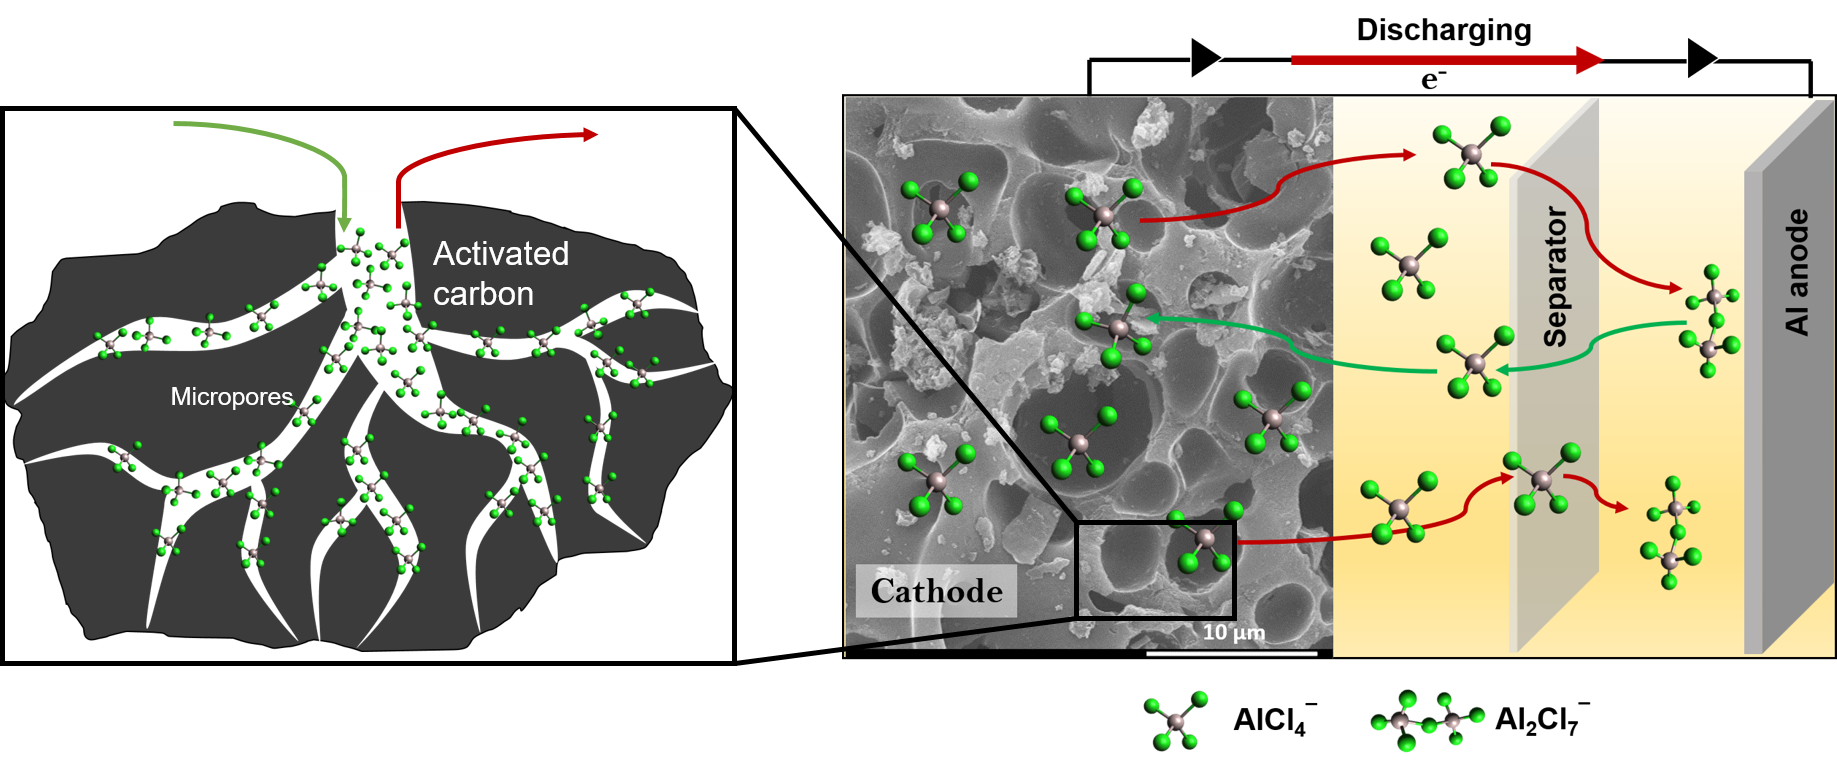
\includegraphics[width=\textwidth]{figures/scheme1}
    \caption{Charge discharge cycles of ACH, hemp fibers, CFEx and Super-P carbon at a current rate of 36 mA g$^-{^1}$}
  \label{figures:fig1}
\end{figure}
% Figure 1 here
\begin{figure}[h]
  \centering
  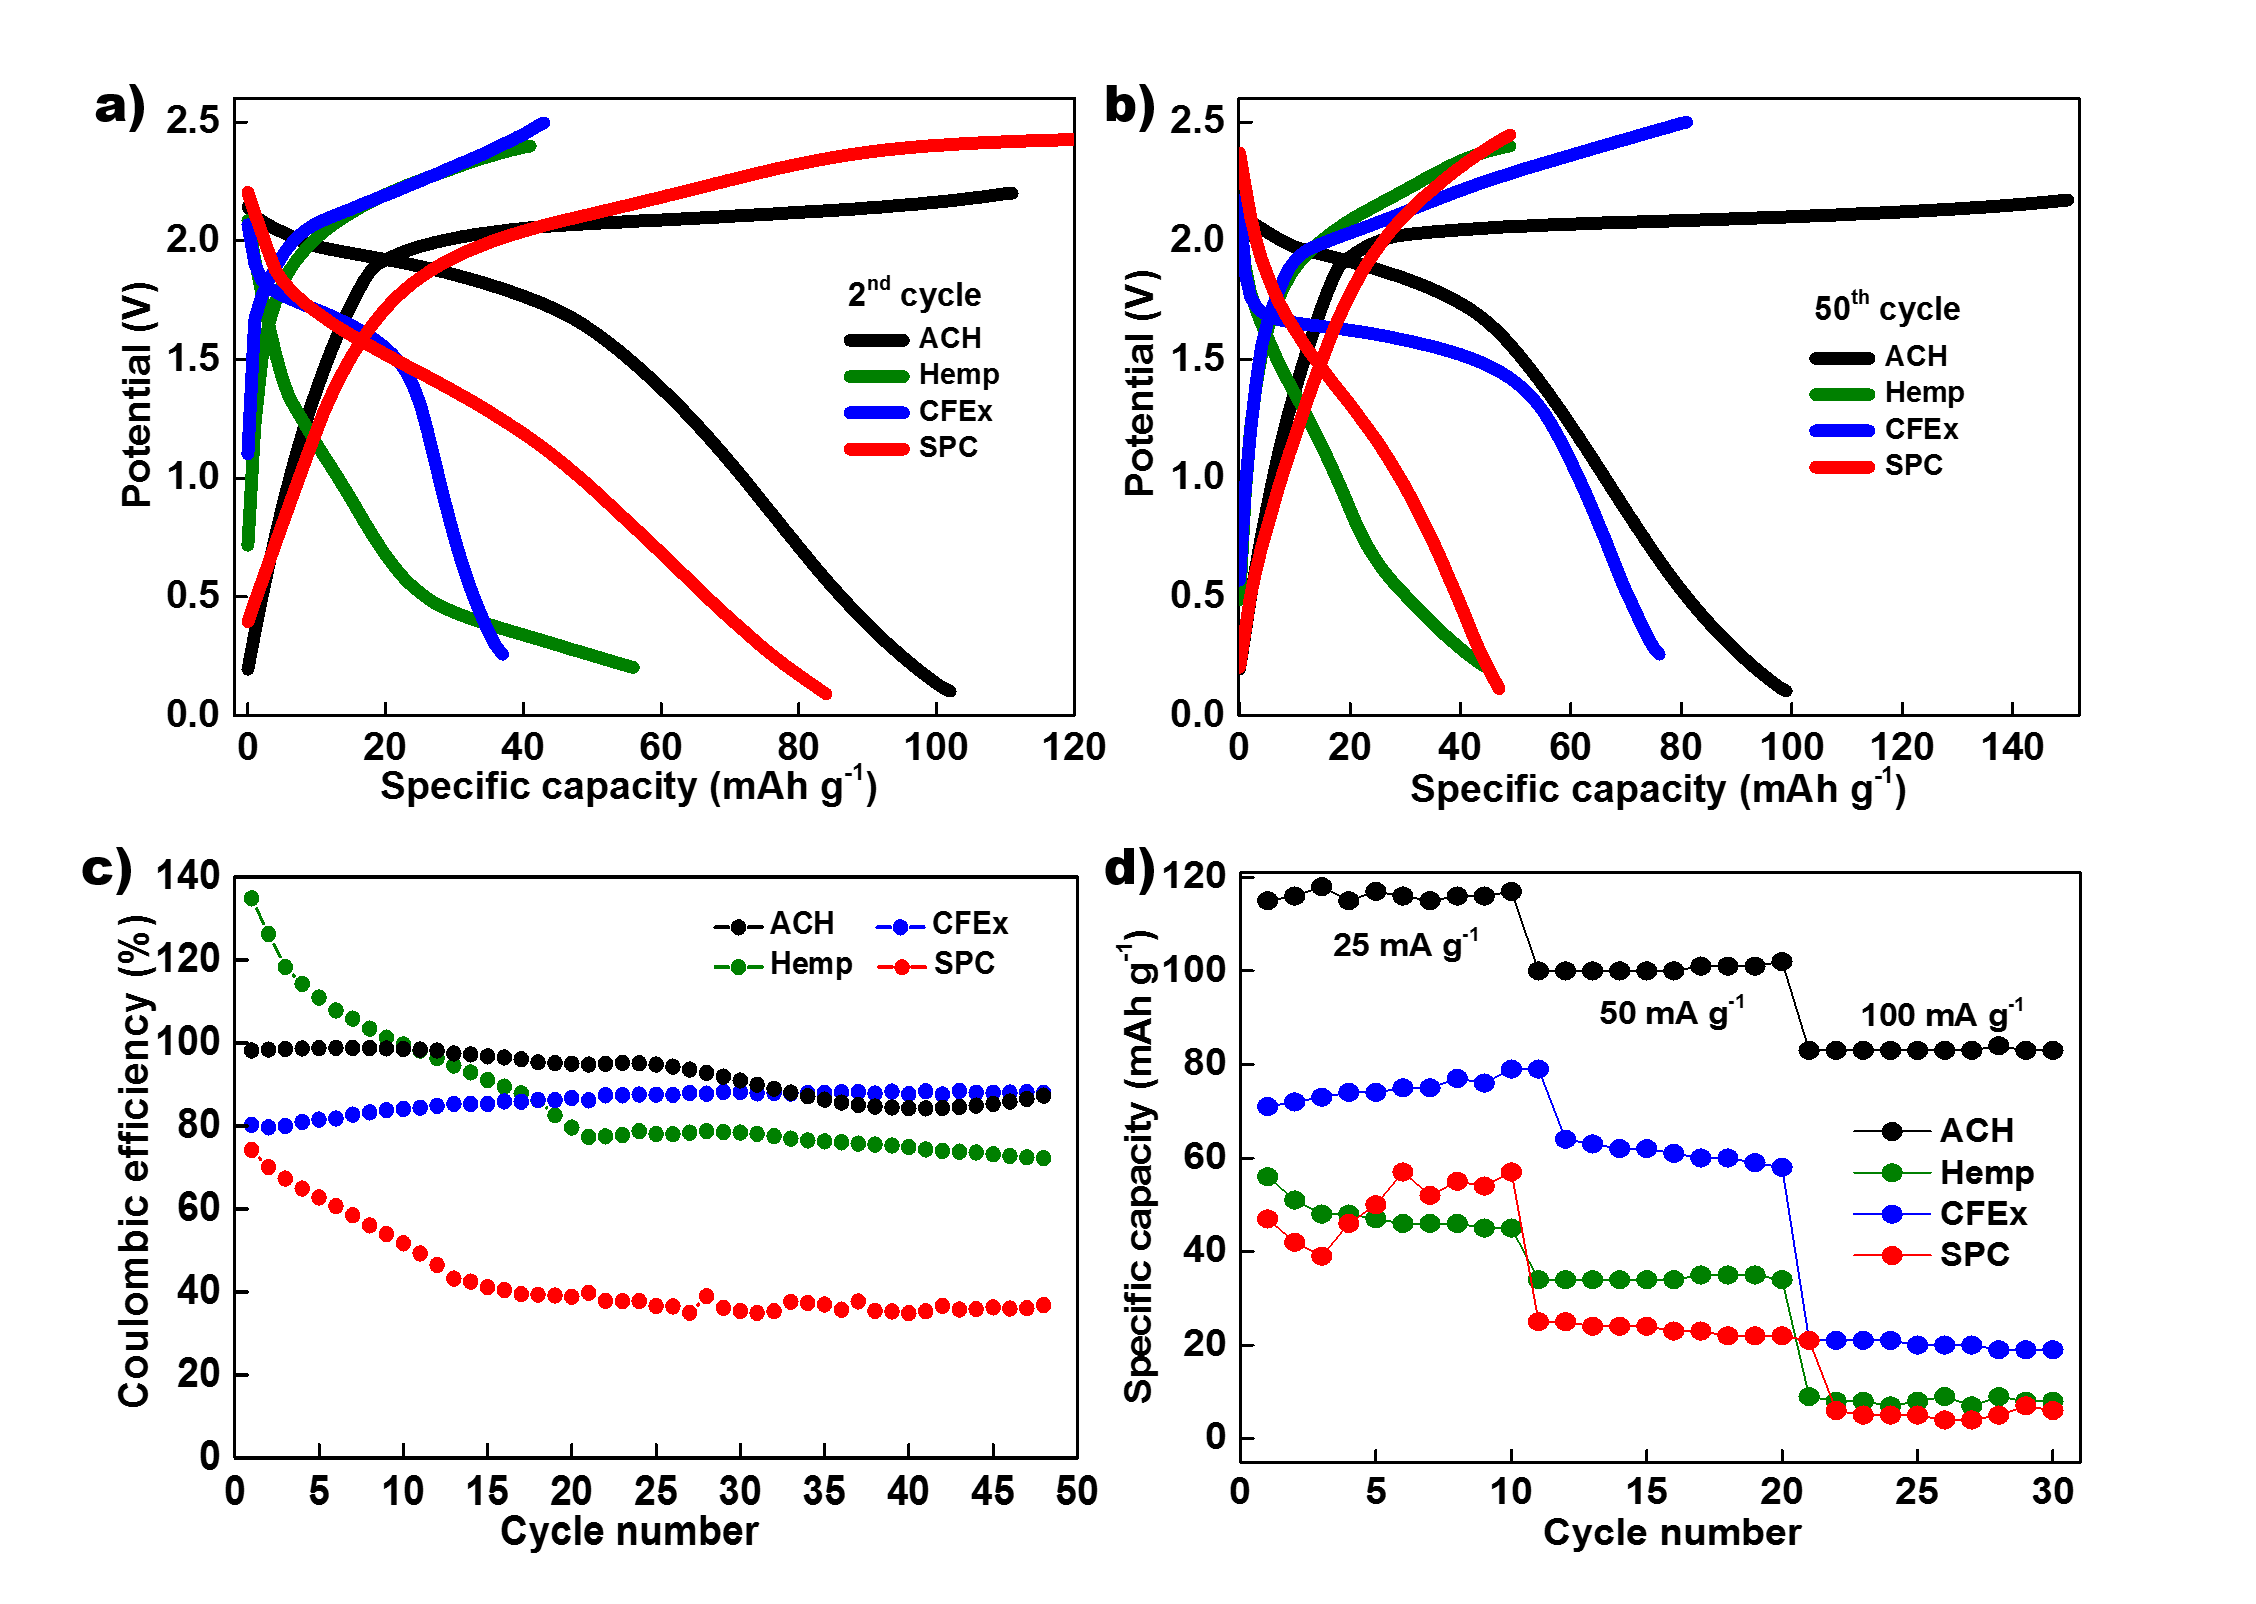
\includegraphics[width=\textwidth]{figures/fig1}
    \caption{Charge discharge cycles of ACH, hemp fibers, CFEx and Super-P carbon at a current rate of 36 mA g$^-{^1}$}
  \label{figures:fig1}
\end{figure}

In this work, we compared different carbon cathodes using pure Al foil as an anode and a room temperature ionic liquid (RTIL) as the electrolyte. Activated carbon, hemp fibers and Super-P carbon cathodes display poorer graphitic structure, which is reflective in the high intensity D-band in their Raman spectra (Figure X). Using a Neware BTS 3000 battery analyser, charge and discharge capacities of the cathodes were recorded at a constant current density of 50 mA g-1. Al/ACH cell recorded its highest discharge capacity at 102 mAh g-1 with a charging capacity of 219 mAh g$^-{^1}$, and maintained its value after 50 charge-discharge cycles with the charging capacity decreasing to . Coulombic efficiency varied for the first few cycles but stabilised in the last few, at ~95\%. This material showed a very stable behaviour indicating absence of cathode degradation. ACH, hemp fibers and Super-P carbon have some graphitic structure present in them (evident from the presence of G-bands in their Raman spectra), we can assume intercalation and deintercalation of ions to take place in those graphitic layers when we charge the cell. Further analysis might help in establishing this hypothesis. A high battery potential (1.92 V) ensures this battery can be used as a cheaper alternative to Al/ graphite cells.  Al/ hemp batteries showed a capacity of 56 mAh g$^-{^1}$ in their first cycle which decreased to 45 mAh g-1 after 50 cycles. Coulombic efficiency for this cell decreased with every cycle, which might indicate self-discharge. Al/ CFEx batteries recorded their first discharge capacity at 37 mAh g$^-{^1}$ which increased to 78 mAh g$^-{^1}$ after 50 cycles. This battery showed a very stable coulombic efficiency at ~90\%. Stability of the cathode before and after cycles was supported by their Raman analysis, X-ray diffraction spectra and SEM images. Al/ SPC cells underwent the highest change while recording their specific capacity. With an initial capacity of 84 mAh g$^-{^1}$, their value decreased to 47 mAh g$^-{^1}$ after 50 cycles.  It displayed a low coulombic efficiency ranging from 75\% to 40\%, which stabilized at ~40\% in the last 30 cycles. This active material is extremely amorphous. They display particle size of ~30 nm, which is 100 times bigger than AlCl$_4{^-}$ ions. SPC has the least graphite-like structure when compared to ACH and hemp fibers. It remains amorphous after the charge-discharge cycles degrading the cathode, which leads to a loss in its specific capacity and coulombic efficiency. It was observed that the cheapest material of the tested samples, ACH, turned out to be the best performing cathode with not only a higher specific capacity than natural graphite, but also a high battery potential and a stable cycle life. Most of the cathodes presented in this work are composed of sp2 carbon atoms. Their bond energy pushes the vibrational frequency to ~1500 cm$^-{^1}$ that is a characteristic G band Raman peak for graphite like carbon atoms. Sharpness of the G band indicates the symmetry of a material. 

% Figure 2 here

\begin{figure}[h]
  \centering
  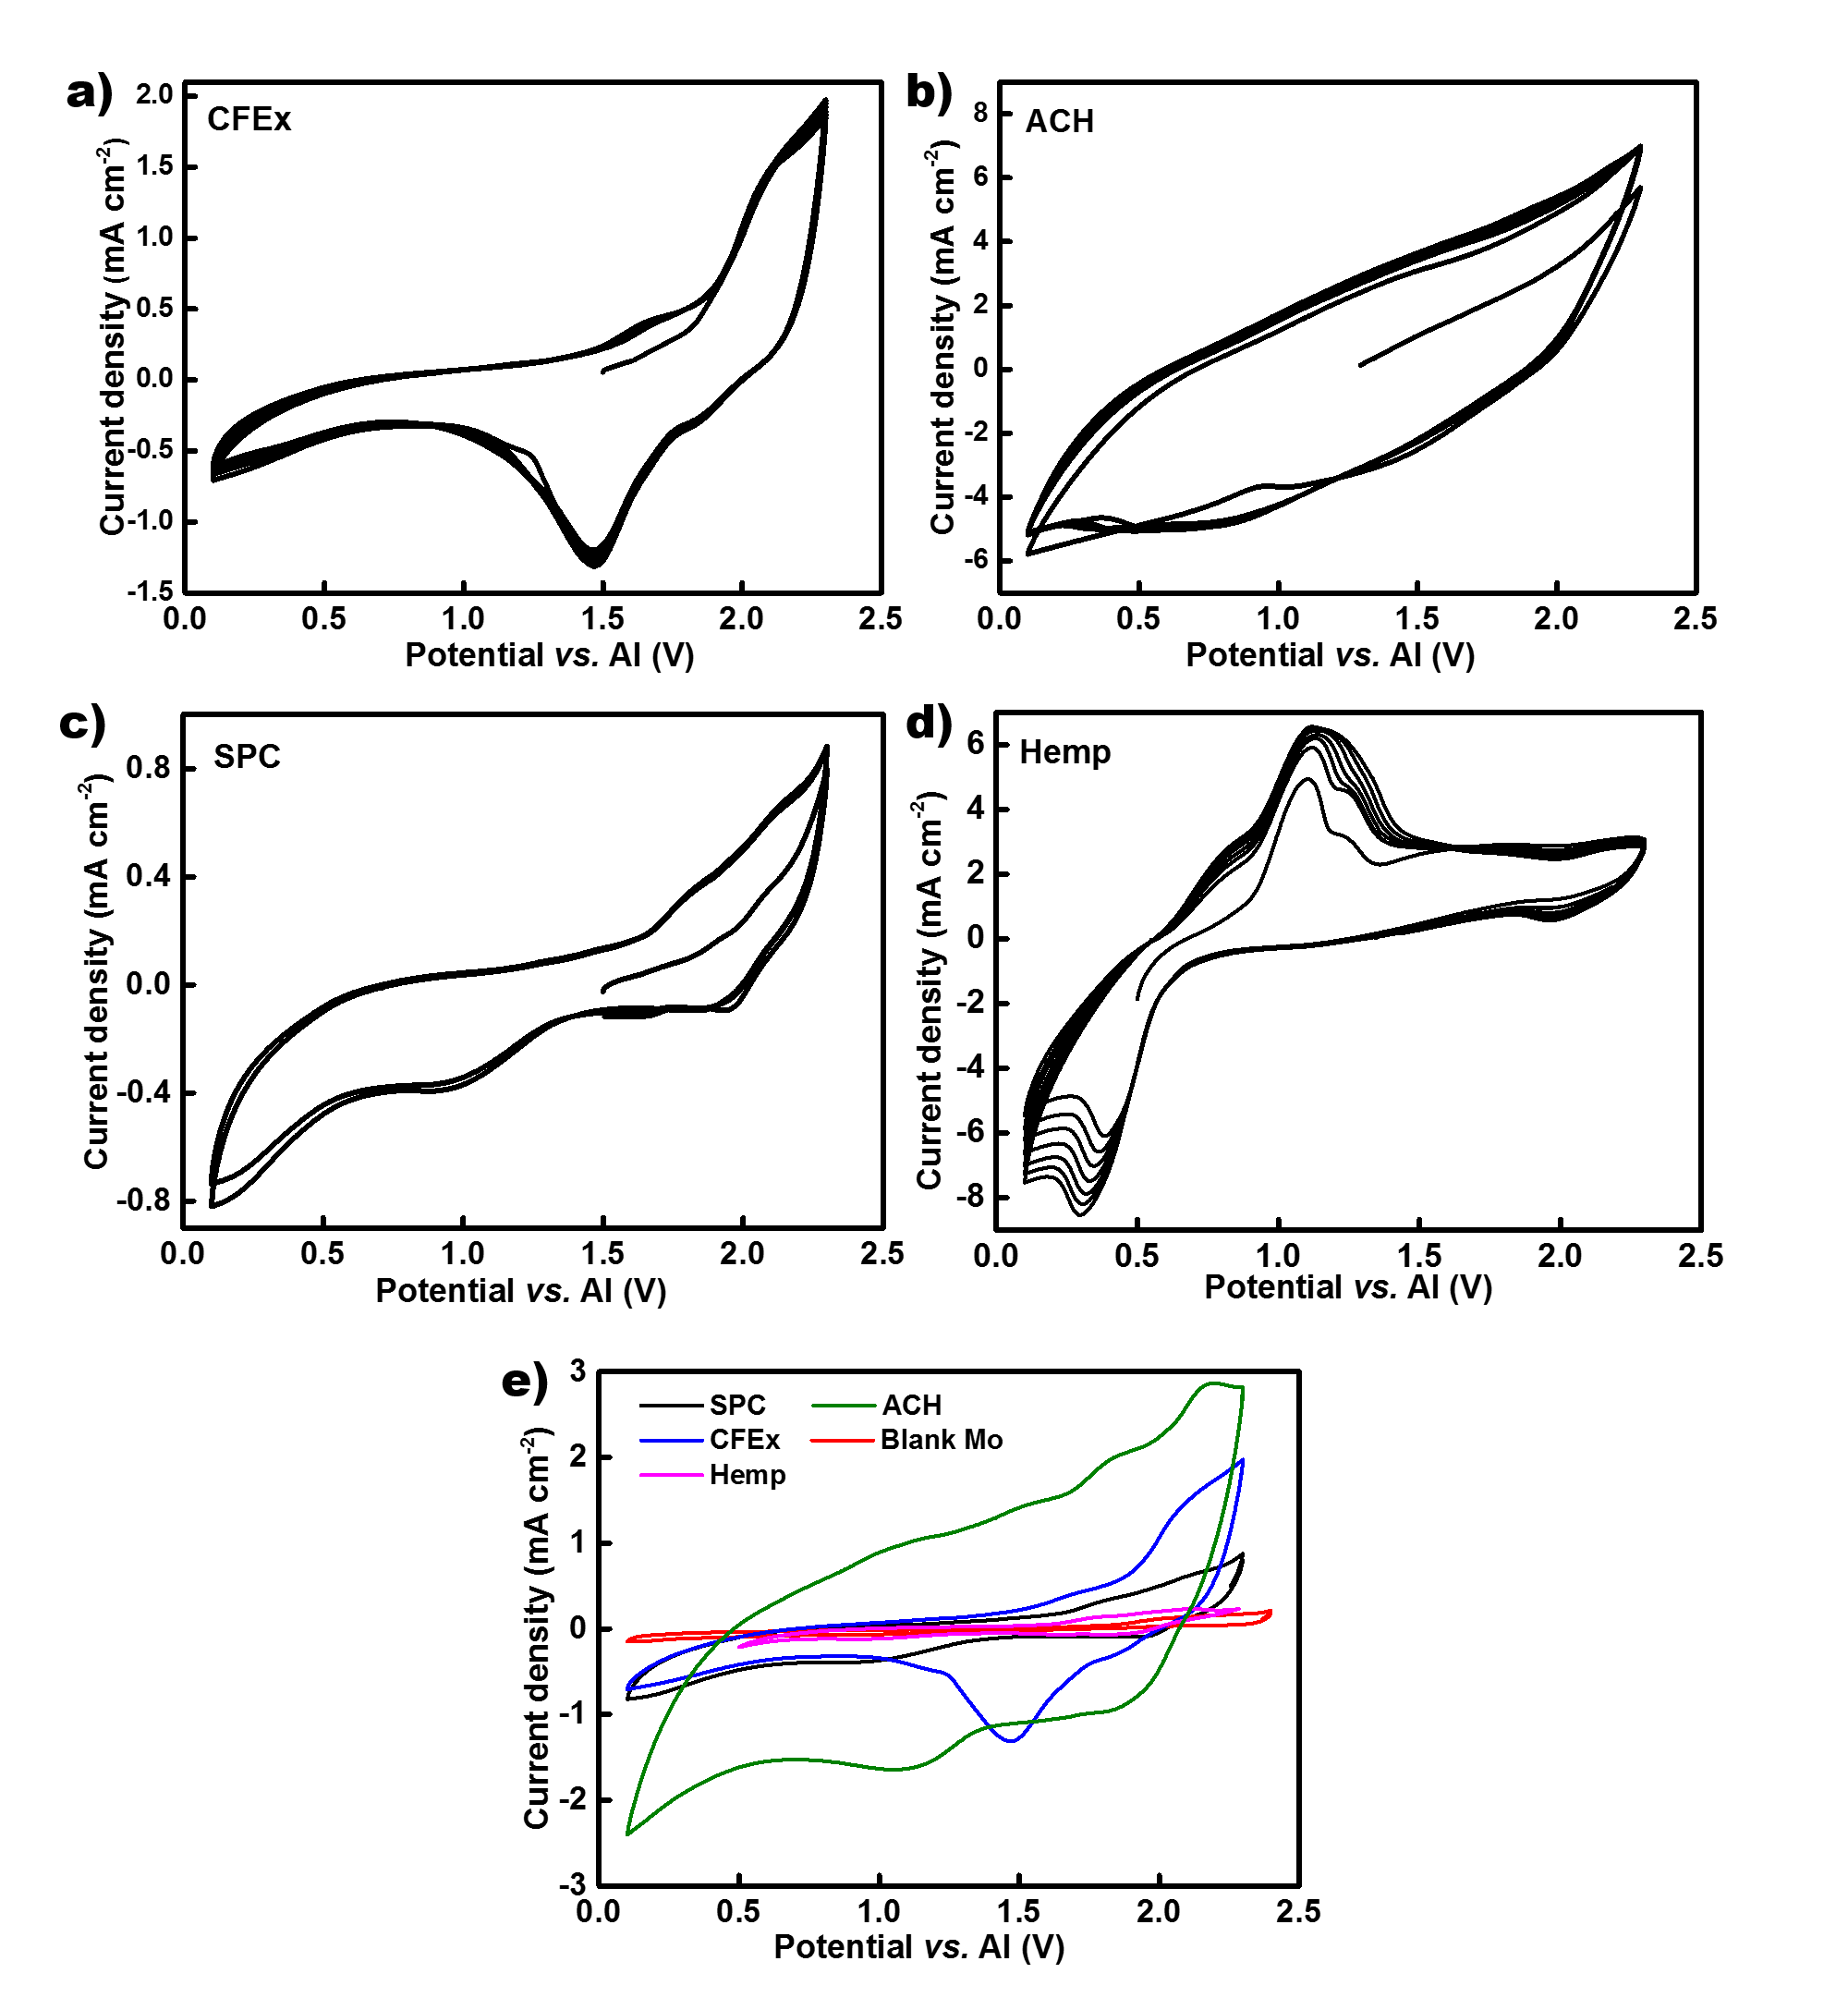
\includegraphics[width=\textwidth]{figures/fig6}
    \caption{Schematic for fullerenes.}
  \label{figures:fig1}
\end{figure}
\begin{figure}[h]
  \centering
  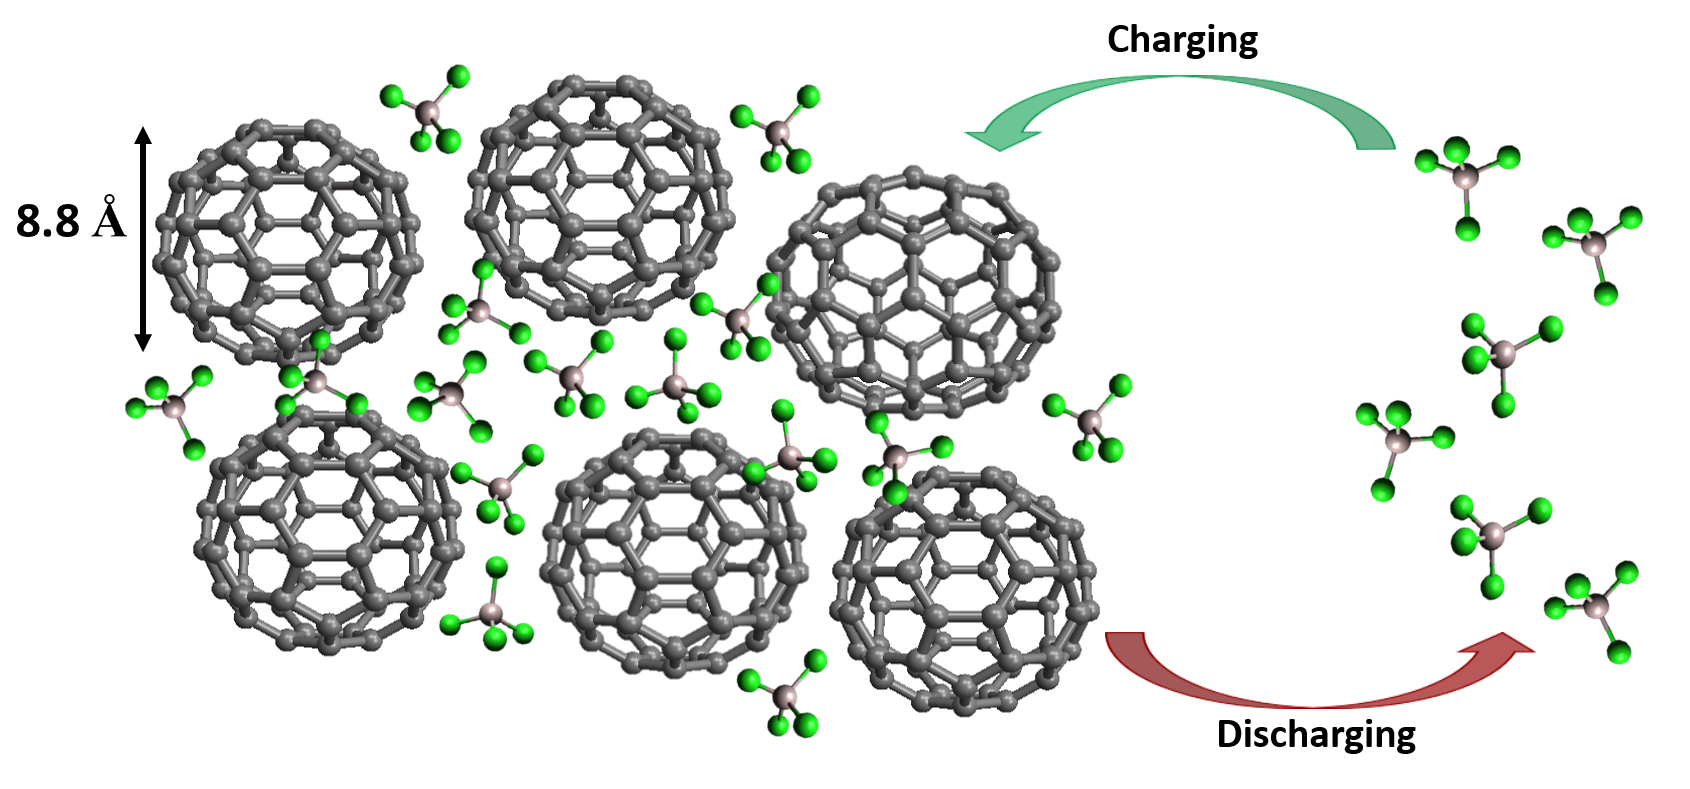
\includegraphics[width=\textwidth]{figures/fig2}
    \caption{Schematic for fullerenes.}
  \label{figures:fig1}
\end{figure}
\begin{figure}[h]
  \centering
  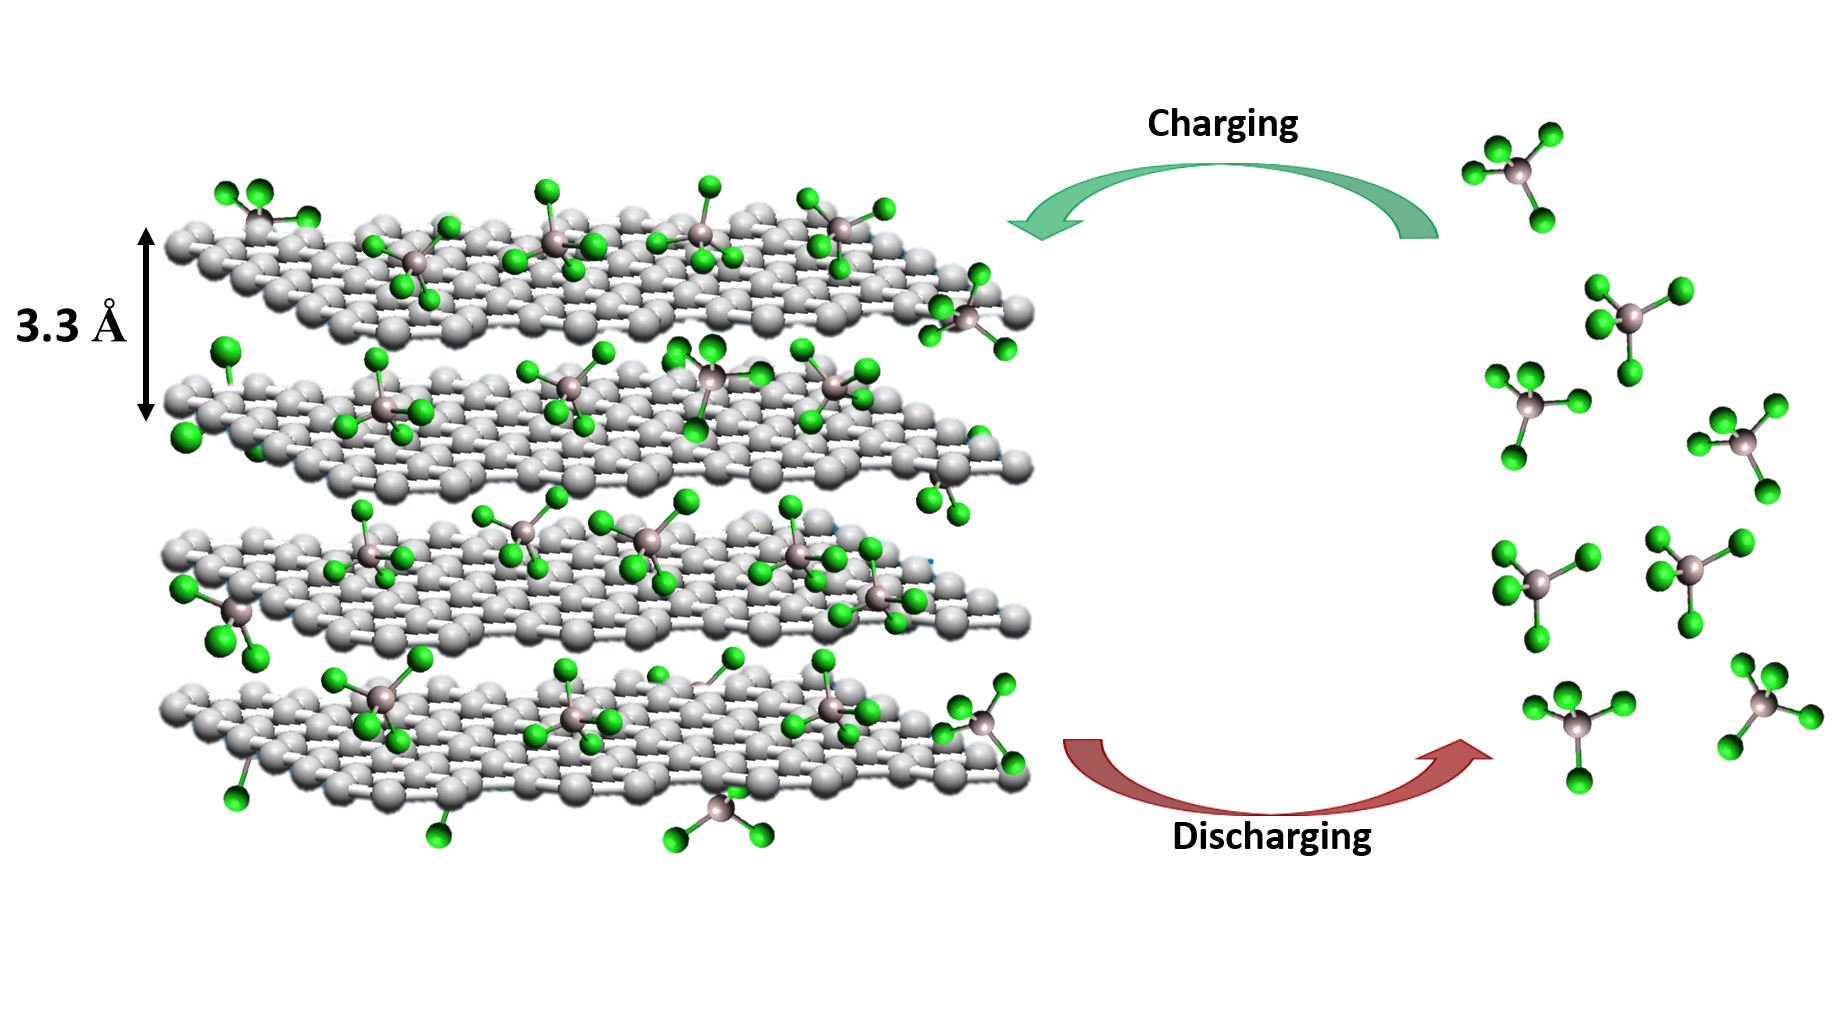
\includegraphics[width=\textwidth]{figures/fig3}
    \caption{Schematic for graphite.}
  \label{figures:fig1}
\end{figure}
\begin{figure}[h]
  \centering
  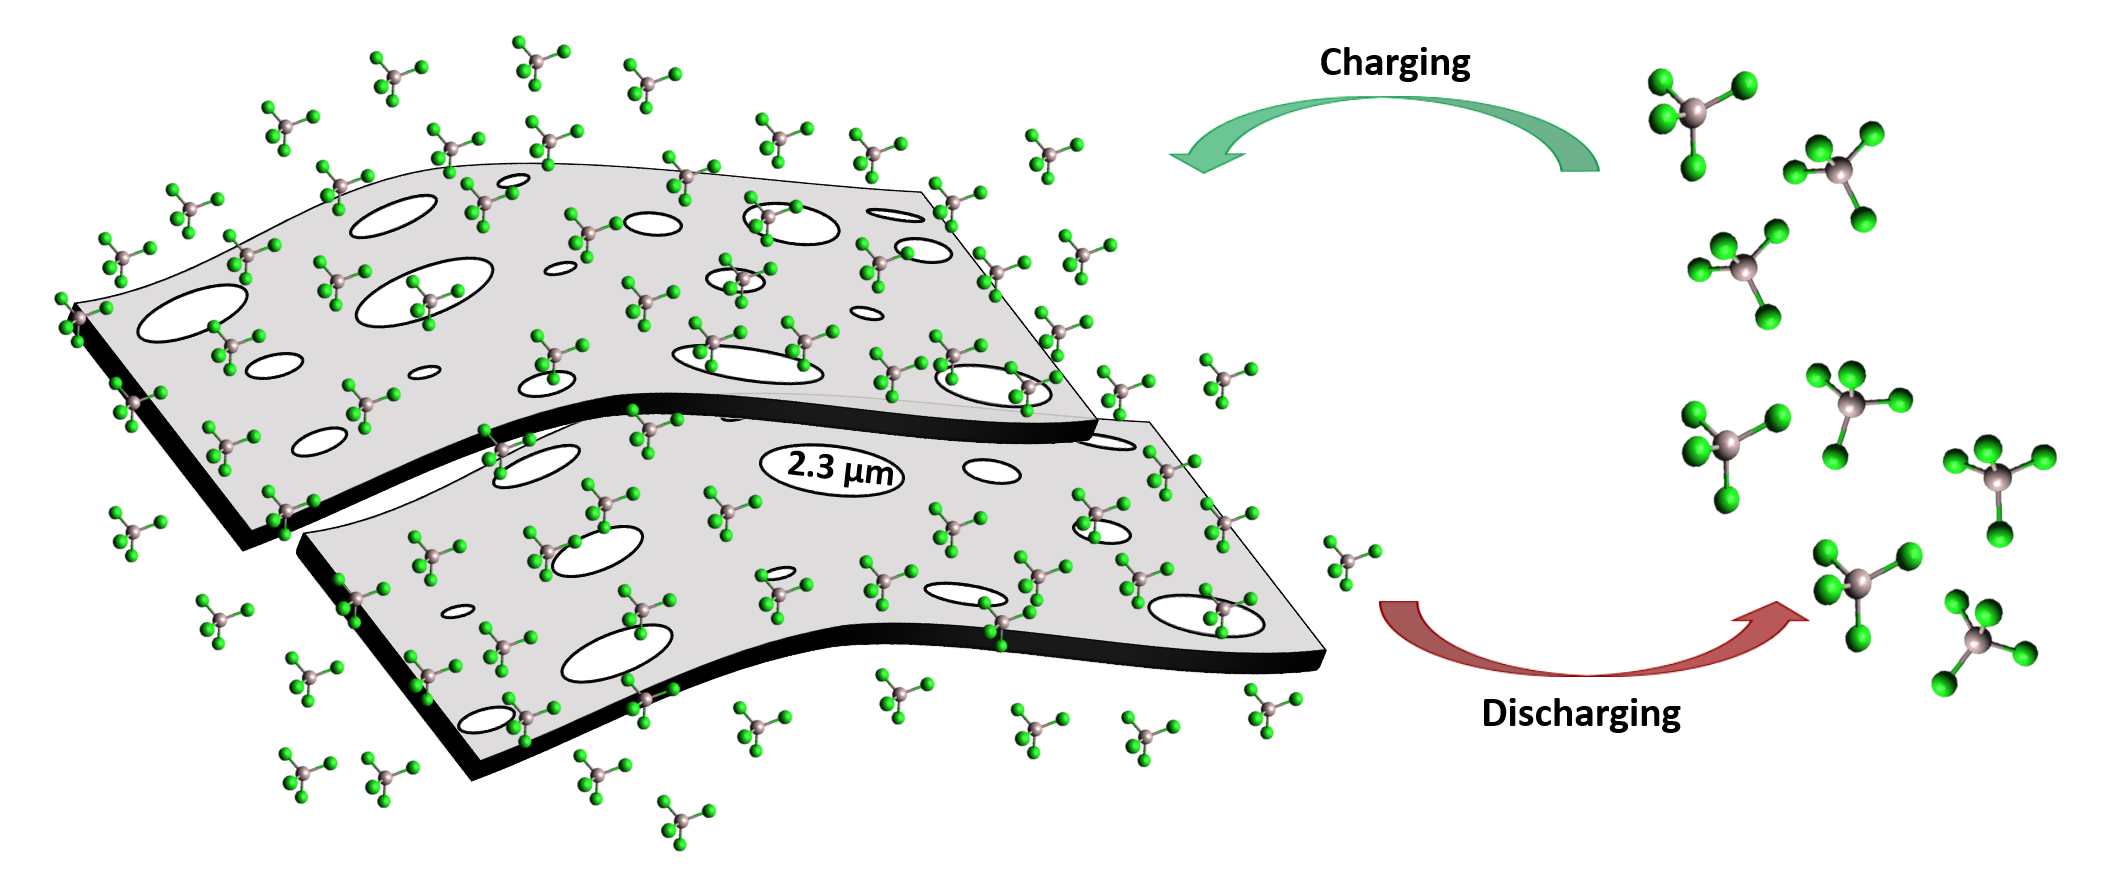
\includegraphics[width=\textwidth]{figures/fig4}
    \caption{Schematic for hemp fibers.}
  \label{figures:fig1}
\end{figure}
\begin{figure}[h]
  \centering
  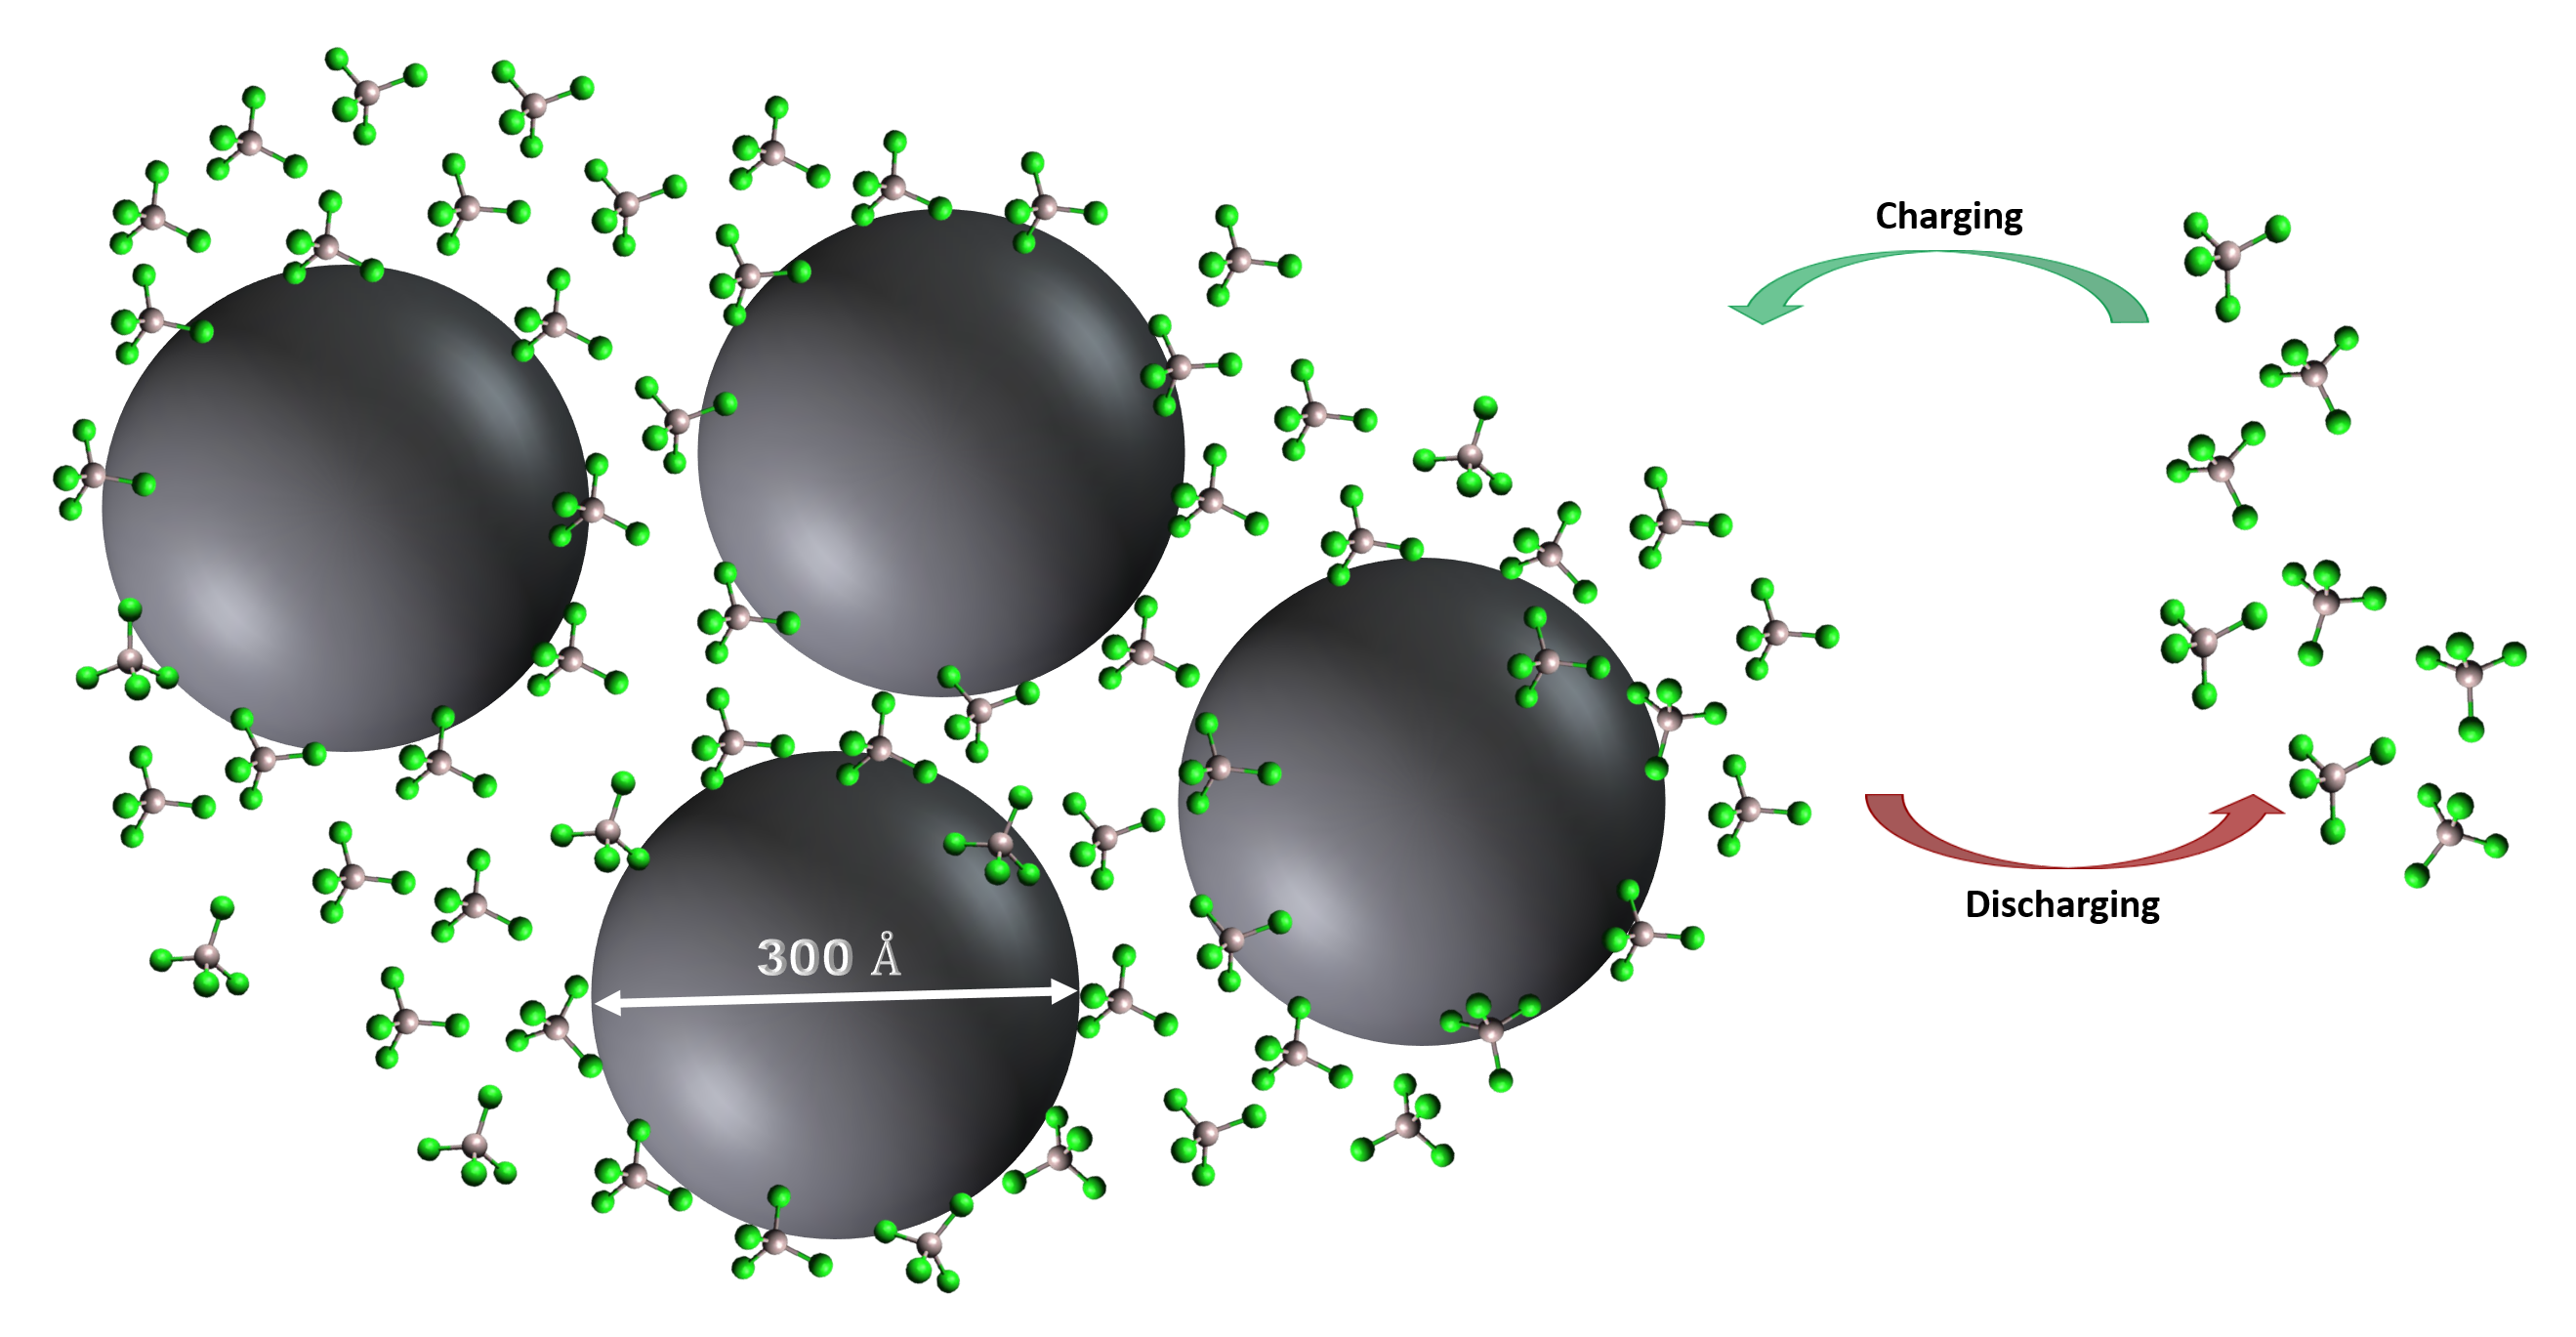
\includegraphics[width=\textwidth]{figures/fig5}
    \caption{Schematic for Super-P carbon.}
  \label{figures:fig1}
\end{figure}
\begin{figure}[h]
  \centering
  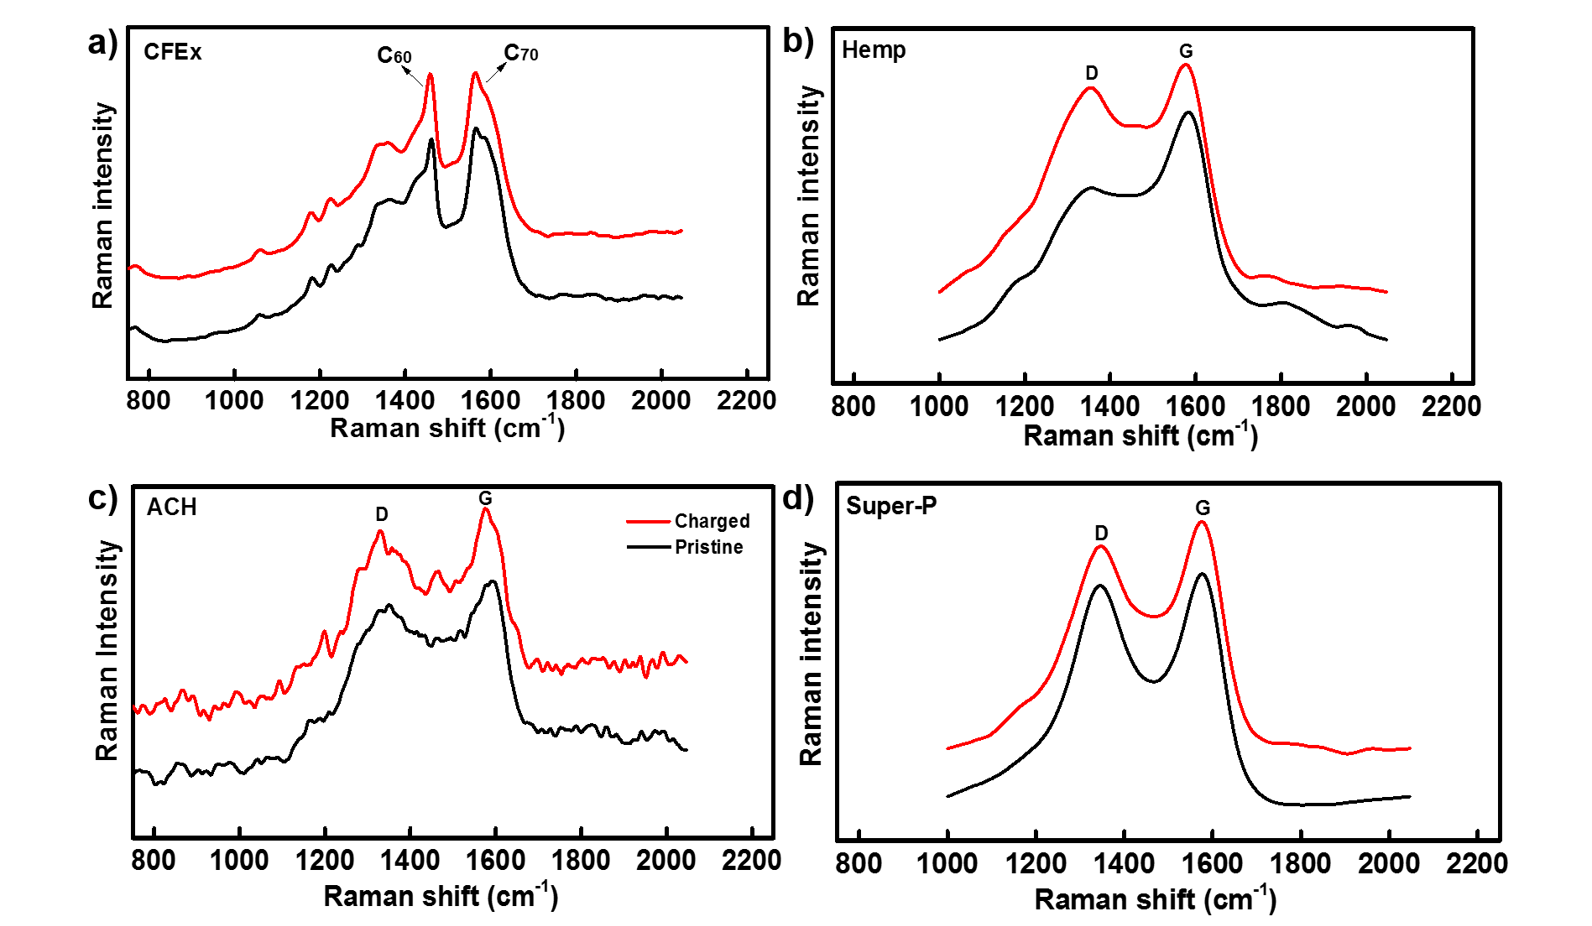
\includegraphics[width=\textwidth]{figures/Raman}
    \caption{Schematic for Super-P carbon.}
  \label{figures:fig1}
\end{figure}
\\Figure 5 illustrates the Raman spectra of the carbon-based cathodes tested here. Most of the pristine samples shown have a significant D-band indicating a non-graphite-like (distorted symmetry) structure.  Activated carbon is amorphous in crystallinity) is significant in both its pristine (black) and charged (red) sample. No major change was observed in the charged cathode showing the stability of cathode structure after charge-discharge cycles. In Figure 5b, we saw that pristine hemp has a sharper G band at 1571.9 cm$^-{^1}$ compared to its charged sample. FWHM (full width at half maximum) of these bands increased after galvanostatic cycles indicating an increase in the amorphous nature of the charged cathodes (see Fig 5a, 5b and 5d). In Figure 5a and 5b, cycled cathodes observed a more intense D band than pristine ones suggesting that cathodes lose their crystallinity with time. ACH, hemp and Super-P have a distinct D band (at ~1300 cm$^-{^1}$) 1329.7 cm$^-{^1}$, 1352.0 cm$^-{^1}$ and 1345.2 cm$^-{^1}$ respectively due to that loss. CFEx on the other hand has its own characteristic peaks owing to different vibrational modes of C60 and C70. Buckyball recorded its characteristic peak at 1459.3 cm$^-{^1}$ (Fig 5c). C$_7{_0}$ has additional peaks due to reduction in its molecular symmetry compared to C$_6{_0}$, increasing the number of active Raman bands. The characteristic band for C$_7{_0}$ shifts to 1560.2 cm$^-{^1}$. An interesting observation is that the pristine and charged samples for CFEx (Fig 5c) have identical Raman spectra indicating the cathode retained its crystalline structure. It suggests that bonds of the sp2 carbon atoms remained unbroken. Another interesting observation in the Raman analysis was a new tiny peak that appeared at 1466 cm$^-{^1}$ for charged ACH cathode (Fig 5a). This new peak can be a result of vibration of C atoms in a plane adjacent to intercalant layer planes. A similar G-band splitting was observed by Wang \textit{et al} while charging natural graphite cathodes. Thus establishing the fact that ACH undergoes a similar mechanism like graphite, where AlCl$_4{^-}$ ions intercalate into the cathode while charging. No such effect was observed for any other cathode. Overall, the Raman analysis revealed ACH and CFEx cathodes to be more stable than the rest, whereas hemp fibers and SPC degraded after a few cycles. 
\begin{figure}[h]
  \centering
  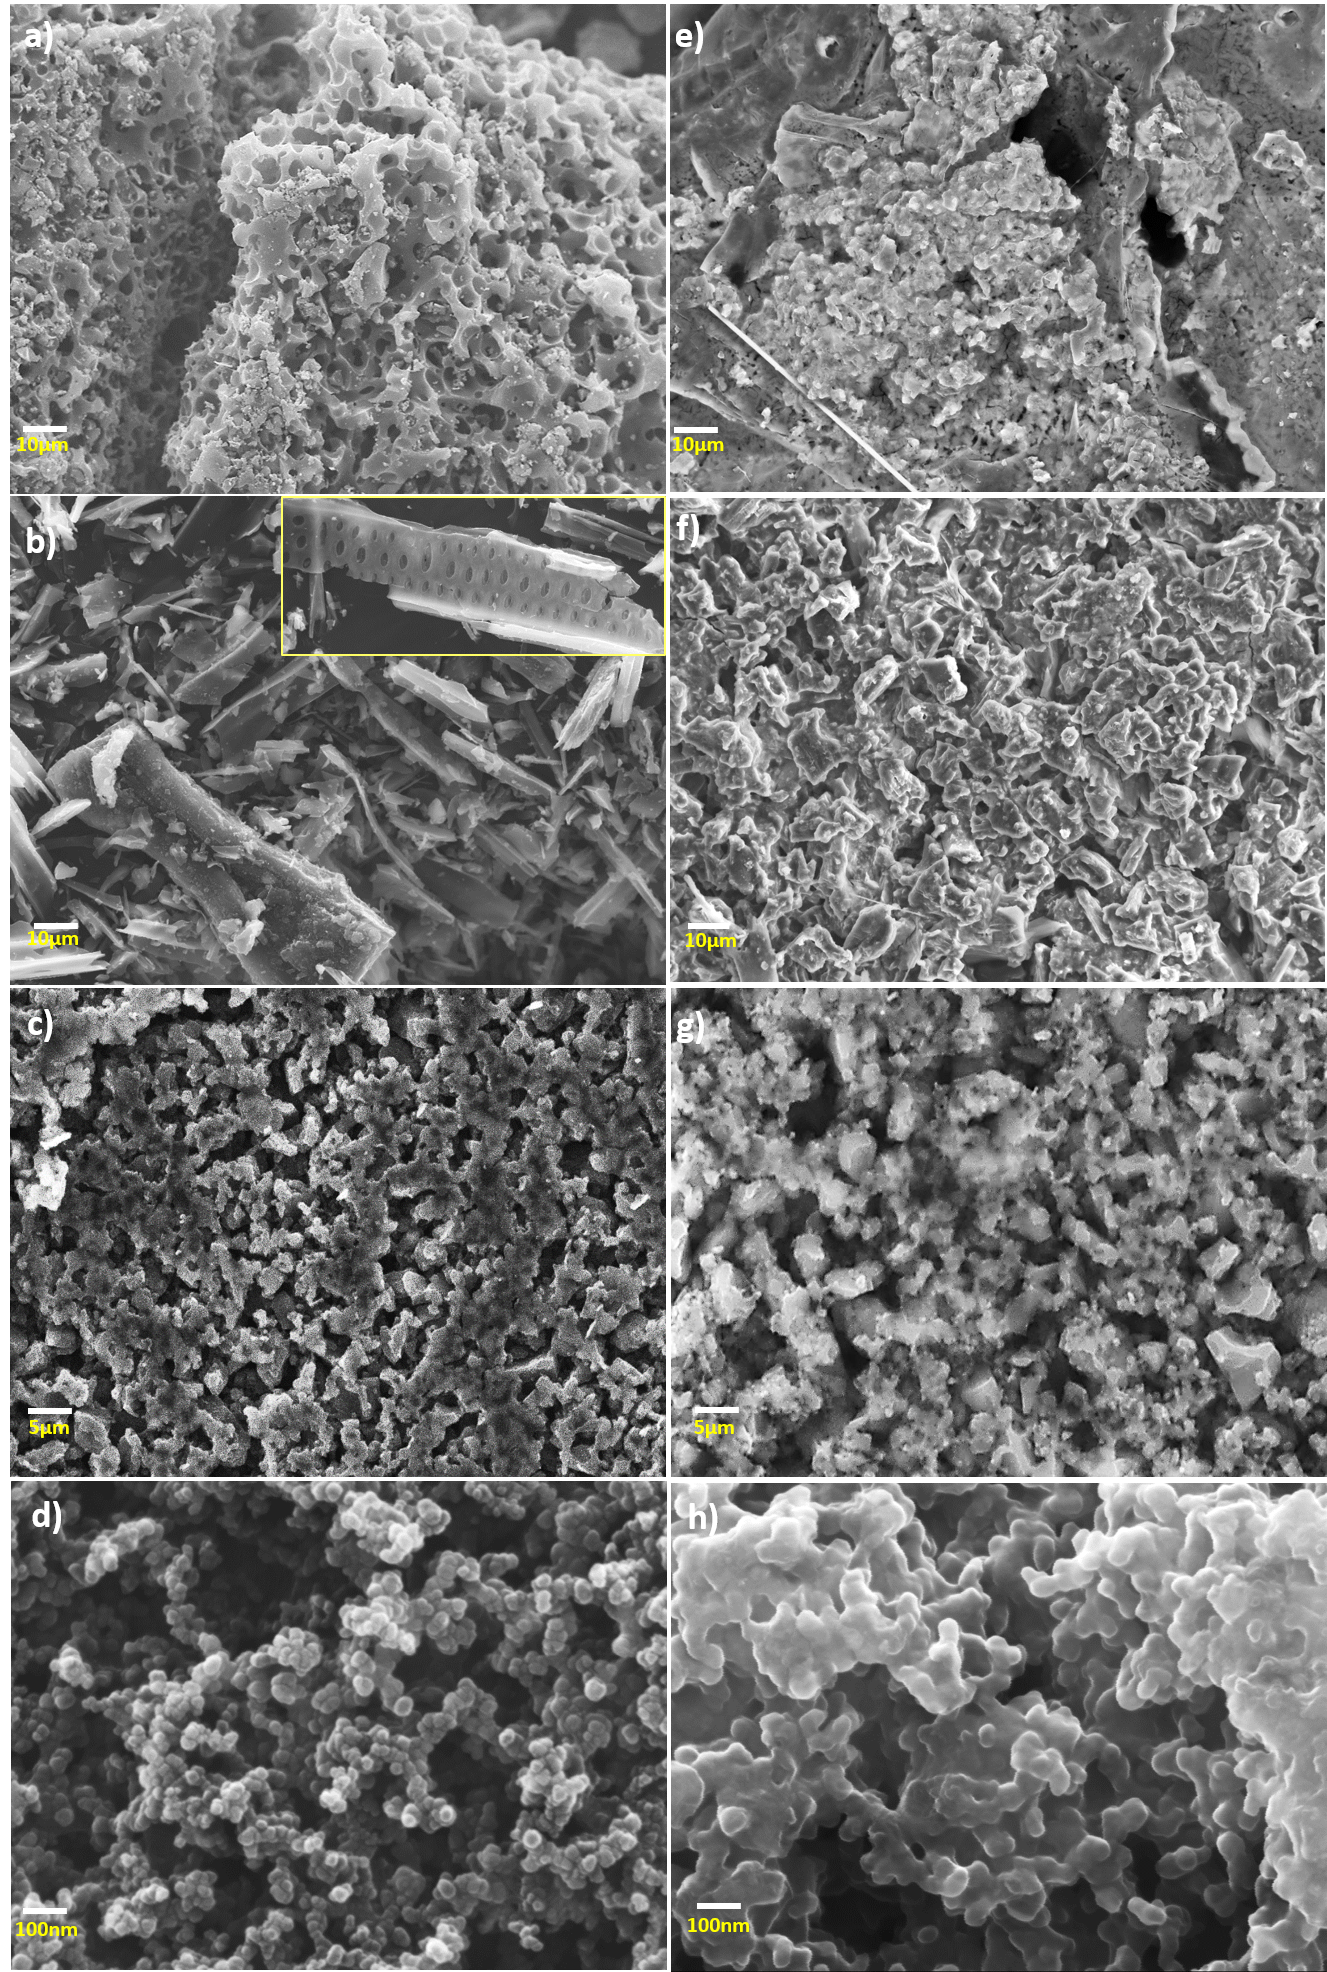
\includegraphics[width=\textwidth]{figures/SEM}
    \caption{Schematic for Super-P carbon.}
  \label{figures:fig1}
\end{figure}
It appears that above results are in good agreement with the SEM images (Figure 6) of the carbon-based cathodes tested here. ACH has a very porous structure (Figure 5a), which is quite similar to the hemp fibres (Figure 6b- picture inset). Figure 6e showed morphology of the charged ACH sample, which did not appear very different from its pristine sample. Figure 6f displayed the SEM image of the charged hemp cathode, which appeared degraded due to agglomeration of the fibers after electrochemical cycles. The images were in accordance with their Raman spectra (Fig 5b). Surface morphology of the fullerenes (Figure 6c and 6g) did not undergo much change, as was evident from its Raman spectra (Fig 5d). This proved that the crystallinity of CFEx remained intact. This evidence was supported by X-ray diffraction spectra of CFEx (Fig S3) where both the charged and pristine samples retained characteristic peaks of C60 and C70 after cycles, suggesting no major structural change in the cathodes. In case of SPC (Fig 6d and 6h), the cathodes appear amorphous before and after; in accordance with their Raman spectra (Fig 5d) which also look similar before and after the cycles. We saw that SEM images established ACH and CFEx as the most stable carbon samples. They did not seem to undergo any significant change in morphology after the galvanostatic cycles. For each of their pristine cathodes, there was an intense D-band peak indicating a non-graphitic structure. CFEx cathode however retained its crystalline structure with identical peak positions of the C60 and C70 molecules after galvanostatic charge/discharge cycles. Hemp and SPC were quite alike in their behaviour. Their coulombic efficiency decreased with every cycle along with capacity decay. ACH proved to be the best carbon-based cathode among all the tested cathodes, with a specific capacity of 100 mAh g$^-{^1}$ maintained for 50 cycles at a potential of 1.9 V with a coulombic efficiency of ~90\%. It is comparable to natural graphite, which has been established as a conventional cathode for aluminium-ion batteries. It has been known for a while that in case of graphite, AlCl$_4{^-}$ ions intercalate the cathode when the cells charge and deintercalate during discharge (Figure 7). ACH, hemp fibers and Super-P carbon have some graphitic structure present in them (evident from the presence of G-bands, Fig 5a, b and d), we can assume that intercalation and deintercalation of ions to take place in those graphitic layers when we charge the cell. CFEx on the other hand lacks a layered structure; it is mainly a cluster of Buckyballs and C$_7{_0}$ molecules. AlCl$_4{^-}$ ions tend to seep in and out of the gaps in between the fullerenes (Figure 8) when we charge and discharge the cells. A few fullerenes expand after the first few cycles, which allows more AlCl$_4{^-}$ ions to seep through leading to a higher capacity indicating an increase in the specific capacity value after 50 cycles. 
Since no actual bonds form between the carbon atoms and AlCl$_4{^-}$ ions, no structural change takes place in the cathode resulting in a similar SEM image before and after the cycles. This can be accounted for the identical Raman spectra recorded before and after the charge-discharge cycles.  Since the cathode structure maintains its mechanical integrity, the coulombic efficiency remains stable throughout the cycles. Hemp fibers and Super-P on the other hand, have a highly amorphous structure. Intercalation of AlCl$_4{^-}$ takes place in between the very few graphitic sheets that are present in these molecules resulting in a low capacity value (Figure 9). The non-defined nature of these materials leads to agglomeration of carbon atoms after every charge (evident from their SEM image, Fig 6b, 6f and 6d, 6h). This reduces the number of AlCl$_4{^-}$ ions that intercalate into those layers, decreasing the capacity value over time. Cathodes degrade after every cycle in case of hemp fibers and SPC, indicated by a decrease in their coulombic efficiency after 50 cycles.  It was observed that ACH-the cheapest material of all, turned out to be the best performing cathode. Figure 10 compares the 50th cycle measurement for AL/ACH and Al/natural graphite cell. It not only displays a higher specific capacity than conventional graphite, but also a high battery voltage of 1.92 V with an energy density of 202 Wh kg$^-{^1}$. 


\section{Experimental Section}
\subsection{Cathode preparation}
Slurry was prepared by mixing MoX$_2$ (85$\%$ by wt.), 9$\%$ binder (PVDF, MTI Corporation) and 6$\%$ Super-P conductive carbon (99+$\%$ metals basis, Alfa Aesar) in N-methyl pyrrolidone NMP (anhydrous, 99.5$\%$, Sigma-Aldrich). It was ‘doctor-bladed’ on molybdenum foil (thickness 0.1 mm, MTI Corporation) and dried in a vacuum oven at 120°C for 12 hours to adhere the slurry on the conductive substrate and evaporate the solvent. Specific loading of hBN was 12 mg cm$^-{^2}$. 
\subsection{Electrolyte preparation}
Anhydrous AlCl$_3$ (Sigma-Aldrich) and EMImCl (97$\%$, Sigma-Aldrich) were mixed in a molar ratio of 1.3:1, at room temperature. EMImCl was baked in vacuum for 24 hours at 100°C to remove residual moisture. Small aliquots of AlCl$_3$ was added to EMImCl after every few minutes. The ionic liquid was stirred for 2-3 hours until a clear brown liquid was obtained. Since the electrolyte is hygroscopic in nature, it was prepared in a N$_2$-filled glove box with <0.1 ppm H$_2$O/O$_2$. 
\subsection{Cell assembly}
PEEK (polyether ether ketone) cells were used for electrochemical measurements. Molybdenum rods were used as current collectors. MoX$_2$ coated on molybdenum foil was used as the cathode and placed at bottom of the cell. Two glass microfibers (Grade GF/F, Whatman) were used as separators. 80µl of the electrolyte was used to wet the separator. Aluminium foil (thickness 0.1 mm, 99$\%$, GoodFellow) used as an anode and placed on top of the separator. The cell was then sealed and wrapped with a paraffin film to avoid any air or moisture contact. It was assembled in a N$_2$-filled glove box. Since this was a two-electrode setup, aluminium foil was used as both counter and reference electrode. The cell was taken out of the glove box and electrochemical measurements were performed. 
\lipsum[5]
\begin{equation}
\xi _{ij}(t)=P(x_{t}=i,x_{t+1}=j|y,v,w;\theta)= {\frac {\alpha _{i}(t)a^{w_t}_{ij}\beta _{j}(t+1)b^{v_{t+1}}_{j}(y_{t+1})}{\sum _{i=1}^{N} \sum _{j=1}^{N} \alpha _{i}(t)a^{w_t}_{ij}\beta _{j}(t+1)b^{v_{t+1}}_{j}(y_{t+1})}}
\end{equation}

\subsubsection{Headings: third level}
\lipsum[6]

\paragraph{Paragraph}
\lipsum[7]

\section{Examples of citations, figures, tables, references}
\label{sec:others}
\lipsum[8] \cite{kour2014real,kour2014fast} and see \cite{hadash2018estimate}.

The documentation for \verb+natbib+ may be found at
\begin{center}
  \url{http://mirrors.ctan.org/macros/latex/contrib/natbib/natnotes.pdf}
\end{center}
Of note is the command \verb+\citet+, which produces citations
appropriate for use in inline text.  For example,
\begin{verbatim}
   \citet{hasselmo} investigated\dots
\end{verbatim}
produces
\begin{quote}
  Hasselmo, et al.\ (1995) investigated\dots
\end{quote}

\begin{center}
  \url{https://www.ctan.org/pkg/booktabs}
\end{center}


\subsection{Figures}
\lipsum[10] 
See Figure \ref{fig:fig1}. Here is how you add footnotes. \footnote{Sample of the first footnote.}
\lipsum[11] 

\begin{figure}
  \centering
  \fbox{\rule[-.5cm]{4cm}{4cm} \rule[-.5cm]{4cm}{0cm}}
  \caption{Sample figure caption.}
  \label{fig:fig1}
\end{figure}

\subsection{Tables}
\lipsum[12]
See awesome Table~\ref{tab:table}.

\begin{table}
 \caption{Sample table title}
  \centering
  \begin{tabular}{lll}
    \toprule
    \multicolumn{2}{c}{Part}                   \\
    \cmidrule(r){1-2}
    Name     & Description     & Size ($\mu$m) \\
    \midrule
    Dendrite & Input terminal  & $\sim$100     \\
    Axon     & Output terminal & $\sim$10      \\
    Soma     & Cell body       & up to $10^6$  \\
    \bottomrule
  \end{tabular}
  \label{tab:table}
\end{table}

\subsection{Lists}
\begin{itemize}
\item Lorem ipsum dolor sit amet
\item consectetur adipiscing elit. 
\item Aliquam dignissim blandit est, in dictum tortor gravida eget. In ac rutrum magna.
\end{itemize}


\bibliographystyle{unsrt}  
\bibliography{zoteroBBT.bib}  %%% Remove comment to use the external .bib file (using bibtex).
%%% and comment out the ``thebibliography'' section.

\end{document}
